\begin{frame}
  \frametitle{The Random Ray Method}
    \begin{columns}
        \column[t]{5cm}
            \begin{itemize}
                \item The Random Ray Method (TRRM) is a modification to the MOC tracking
                    algorithm.
                \item Track direction and starting position are randomly sampled, ray-traced
                    on-the-fly through geometry during runtime.
                \item Eliminates need to pre-compute and store tracks in memory, efficiently
                    scales into 3D geometries. 
            \end{itemize}
        \column[t]{5cm}
            \begin{figure}[htbp!]
              \begin{center}
                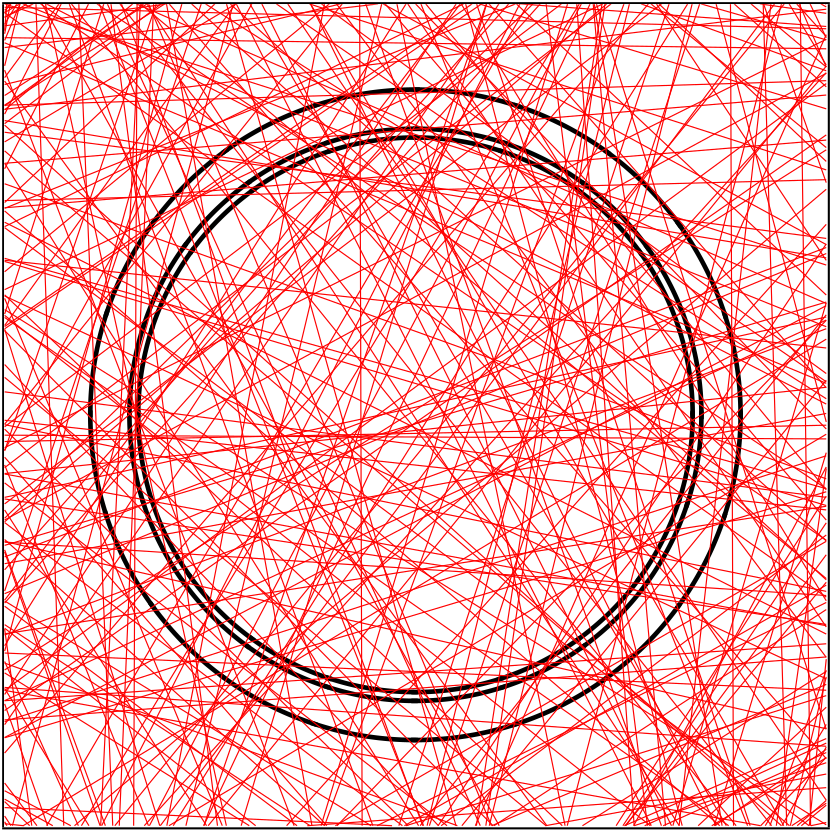
\includegraphics[height=4cm]{./figs/tramm-csg-rr.png}
              \end{center}
              \caption{Randomly sampled tracks used in TRRM. Reproduced from \cite{tramm_development_2018}.}
              \label{fig:moc-tracks}
            \end{figure}
      \end{columns}
\end{frame}
